\chapter{Evaluation}
We have used a machine learning toolkit named as GRT to recognize hand gestures using skeletal points tracking algorithm and Adaptive Naive Bayes classifier (ANBC) for classification and prediction. 

The classifier is based on a statistical model of x,y,z coordinate positions of static hand gestures and provides a likelihood measure for recognized gesture. Furthermore, the gesture recognition pipeline uses two post processing modules such as Class Label Filter and Class Label Change Filter to exclude lower frequent spikes in the prediction results and trigger an output only when there is a change in prediction.

In this chapter, we present the experiments carried out to evaluate and validate our system to recognize hand gestures using skeletal points. The goal is to demonstrate the effectiveness of the classifier and to evaluate its potential for real time input at 30 fps. In the classification phase, input samples are normalized using Min-Max Scaling and Null Rejection is enabled to detect non-gestures. Therefore, the evaluation consists of computing the prediction accuracy for various null rejection coefficient and compare it with other supervised learning classifiers such as Support Vector Machine (SVM).

\section{Mean and Standard Deviation}
ANBC is a supervised learning algorithm that can be used to classify any type of N-dimensional signal. It fundamentally works by fitting an N-dimensional Gaussian distribution to each class when it is trained.

During the training phase, first all the input samples are normalized using Min-Max Scaling with the range from 0 to 1 and then GRT computes mean $\mu$ and standard deviation $\sigma$ to create a model for each class. During the prediction phase, it basically computes the maximum a posterior probability of an input vector belonging to any of the trained class. Figure \ref{fg:ev:mean} shows the mean positions of left and right hand for every gesture. Table \ref{tb:ev:mean} and \ref{tb:ev:sd} show mean and standard deviations of the labeled training data of all the five classes. 

\begin{figure}
	[h]
	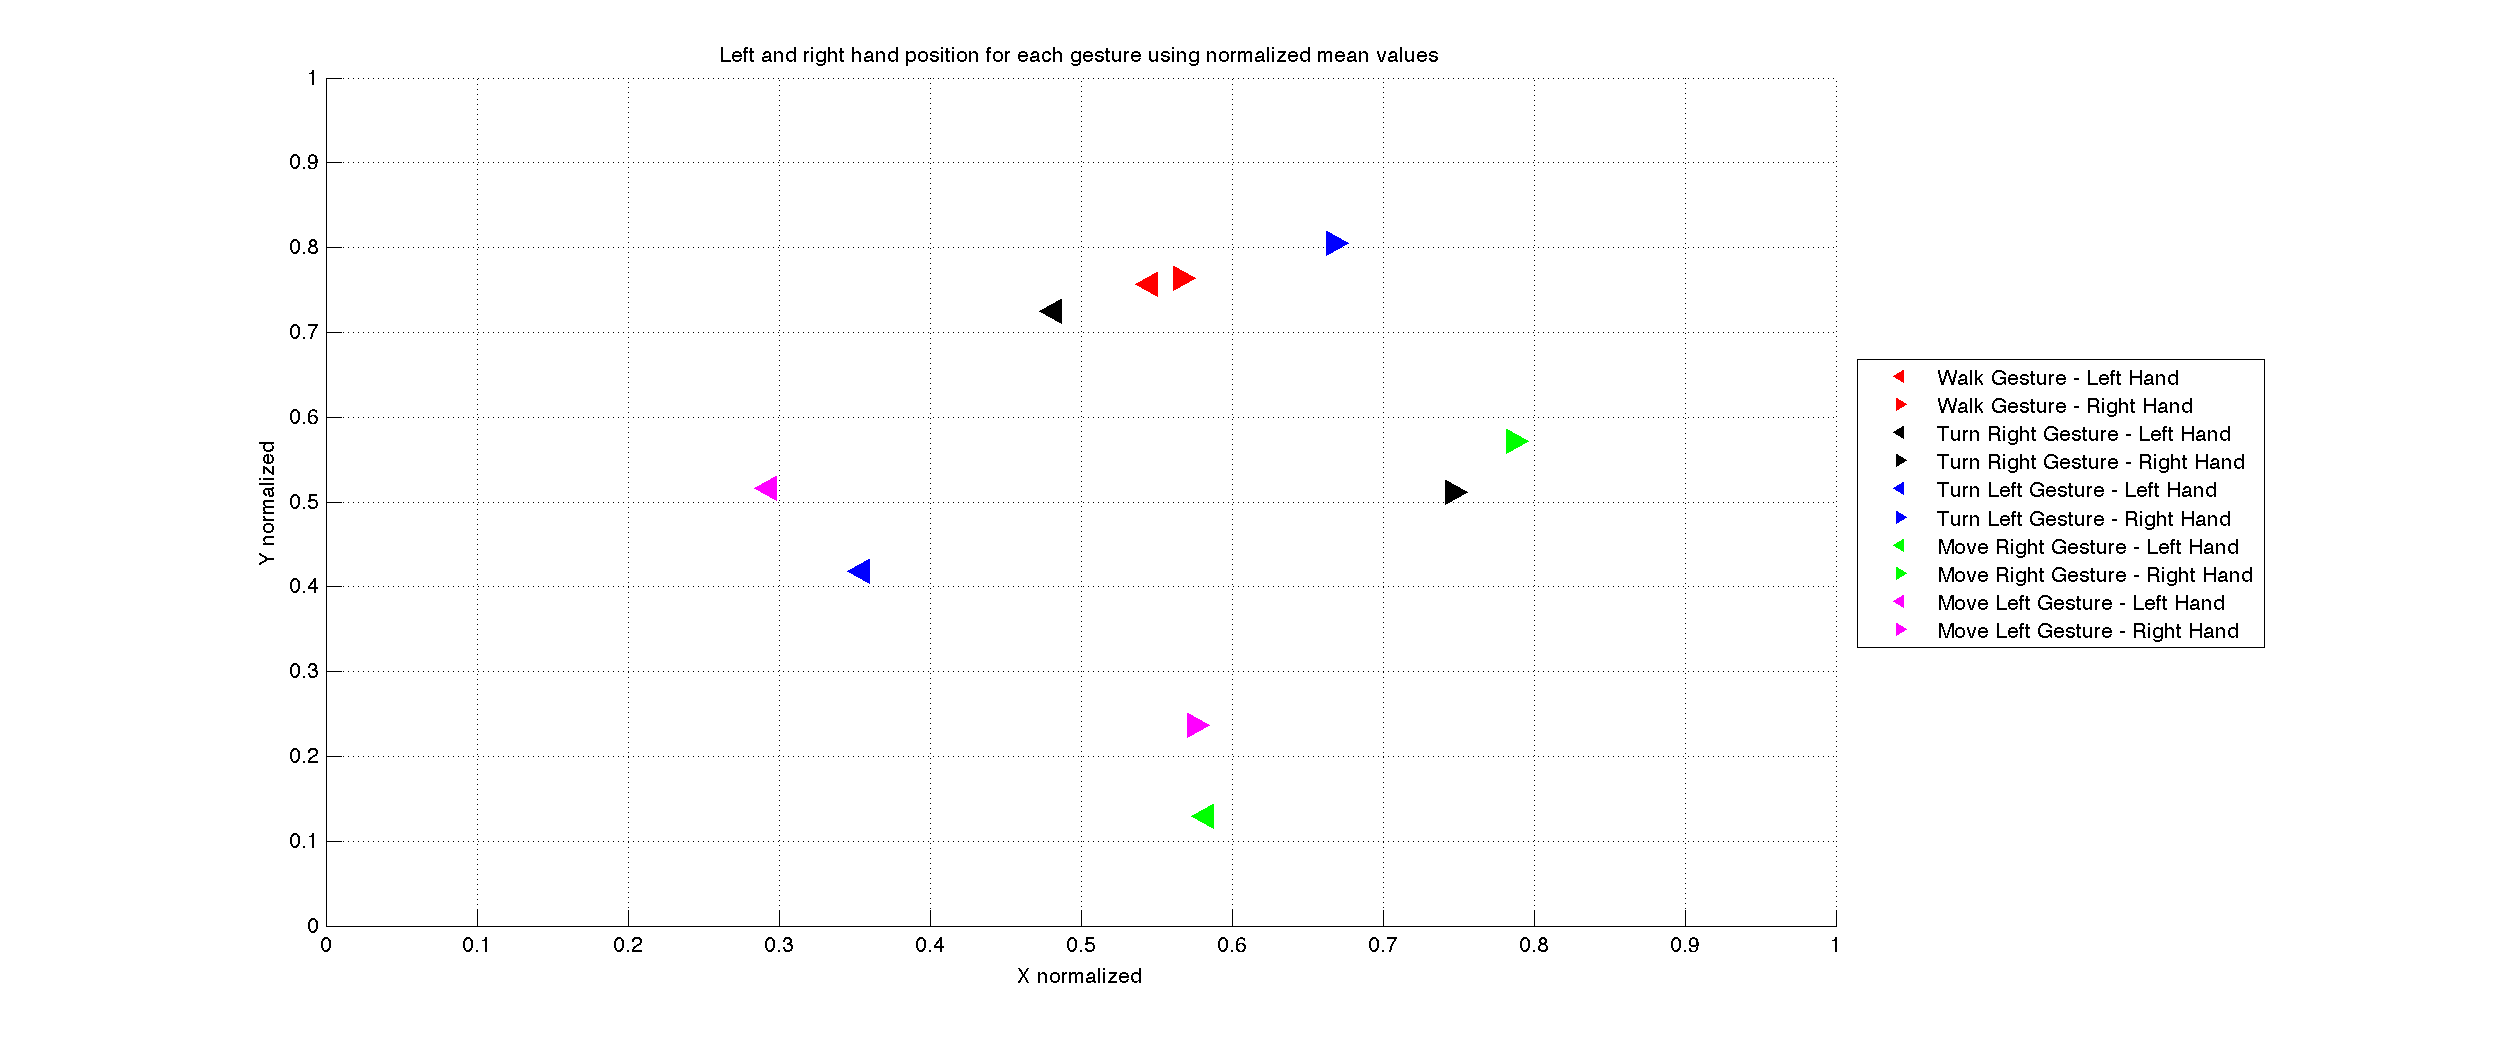
\includegraphics[height=70mm]{/result/train-all-ges-mean.png} \caption{Left and right hand position for each gesture using normalized mean values} \label{fg:ev:mean} 
\end{figure}


\begin{table}
	\centering
	\pgfplotstabletypeset [ col sep=comma, every head row/.style={before row=\hline,after row=\hline}, every last row/.style={after row=\hline}, ] {../../data/results/mean.csv}
	\caption{Normalized mean values of 3 dimensions of left and right hand} \label{tb:ev:mean} 
\end{table}

\begin{table}
	\centering
	\pgfkeys{/pgf/number format/.cd,fixed,fixed zerofill,precision=3}
	\pgfplotstabletypeset [ col sep=comma, every head row/.style={before row=\hline,after row=\hline}, every last row/.style={after row=\hline}, ] {../../data/results/sd.csv} \caption{Standard deviations of 3 dimensions of left and right hand} \label{tb:ev:sd} 
\end{table}

\begin{table}
	\centering
		\pgfkeys{/pgf/number format/.cd,fixed,fixed zerofill,precision=3}
	\pgfplotstabletypeset [ 
	col sep=comma, 
	every head row/.style={before row=\hline,after row=\hline},
	every last row/.style={after row=\hline},
	create on use/newcol/.style={
		create col/set list={Precision,Recall,F-measure}
	},
	columns/newcol/.style={string type},
	columns={newcol,0,1,2,3,4},
	display columns/0/.style={column name={}},
	display columns/1/.style={column name={Class 1}},
	display columns/2/.style={column name={Class 2}},
	display columns/3/.style={column name={Class 3}},
	display columns/4/.style={column name={Class 4}},
	display columns/5/.style={column name={Class 5}},
	] 
	{../../data/results/subset-test/anbc2-precision-recall-fmeasure.csv}
	\caption{Precision, Recall and F-Measure calculated by validating 10\% of training dataset. ANBC Classifier trained with Null Rejection coefficient 2.0} \label{tb:ev:confusion} 
\end{table}


\begin{table}
	\centering
	\pgfkeys{/pgf/number format/.cd,fixed,fixed zerofill,precision=3}
	\pgfplotstabletypeset [ 
	col sep=comma, 
	every head row/.style={before row=\hline,after row=\hline},
	every last row/.style={after row=\hline},
	create on use/newcol/.style={
		create col/set list={Non-gesture,Class 1,Class 2,Class 3,Class 4,Class 5}
	},
	columns/newcol/.style={string type},
	columns={newcol,0,1,2,3,4,5},
	display columns/0/.style={column name={}},
	display columns/1/.style={column name={Non-Gesture}},
	display columns/2/.style={column name={Class 1}},
	display columns/3/.style={column name={Class 2}},
	display columns/4/.style={column name={Class 3}},
	display columns/5/.style={column name={Class 4}},
	display columns/6/.style={column name={Class 5}},				
	] 
	{../../data/results/subset-test/anbc2-confusion.csv}
	\caption{Confusion Matrix calculated by validating 10\% of training dataset. ANBC Classifier trained with Null Rejection coefficient 2.0} \label{tb:ev:confusion} 
\end{table}




\section{Prediction Test}